\section{Contraintes}
Réalisation d'un effet \emph{fisheye} en flex. L'idée est d'appliquer l'effet sur les conteneur présents dans le conteneur appliquant le layout \emph{fisheye}, sous la forme d'une grille dont les éléments grandisse en fonction de la proximité avec la souris.

Dans l'idéal, l'effet produit doit minimiser l'espace entre les conteneurs.

\section{Analyse \& implémentation}

Nous avons fait le choix de créer un layout \emph{fisheye} assurant les traitements nécessaire à la réalisation de l'effet. Pour cela, nous avons utilisé le namespace spark permettant de dissocier le container du layout. Il sera ainsi possible d'associer le layout personnalisé à n'importe quel container spark. Le layout appliquera l'effet sur tous les container dont le container parent est celui sur lequel est appliqué le layout \emph{fisheye}.

Pour la réalisation de ce layout, nous avons eu deux approches qui sont détaillées ci-après.

\subsection{Approche globale}
Cette approche suppose qu'il est possible, en connaissant la position de la souris et la position d'un bloc, de le placer et le dimensionner exactement sur la grille. Les caractéristiques du bloc ne dépendent donc pas du placement des autres blocs voisins.

Le layout peut être paramétré de la manière suivante :

\begin{description}
  \item[maxSize] Taille maximum de l'élément dans la grille,
  \item[minSize] Taille minimum de l'élément dans la grille,
  \item[spread] Propagation de l'agrandissement autour de la souris,
\end{description}

Ainsi le layout va initialiser les éléments sur une grille de la manière suivante :
\begin{figure}[H]
  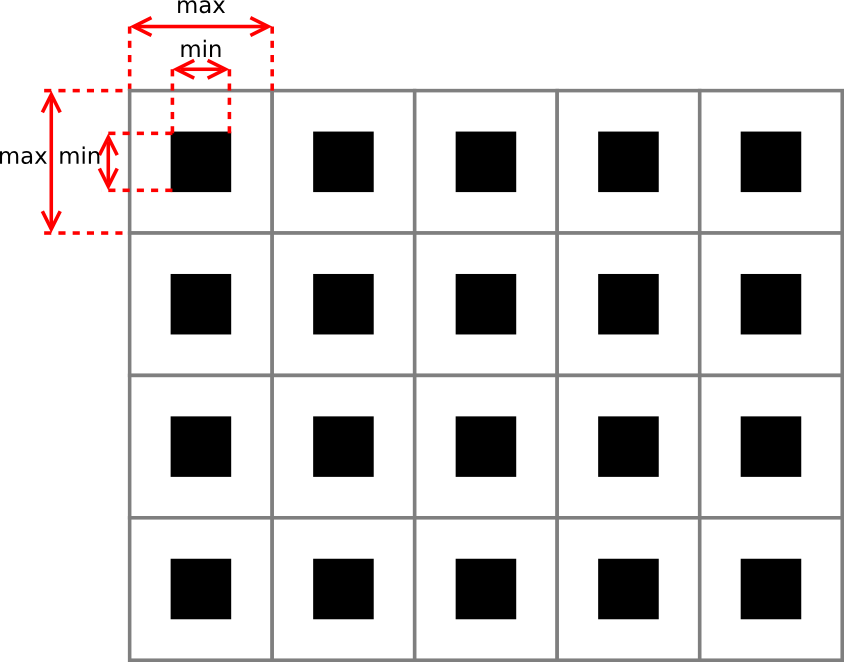
\includegraphics[width=\textwidth]{../resources/illustrations/grob_app_init}
\end{figure}


\subsection{Approche propagée}